\documentclass[10pt,a4paper,UTF8]{article}
\usepackage{zclorg}
\author{emacsun}
\date{}
\title{递归问题:约瑟夫问题}
\hypersetup{
 pdfauthor={emacsun},
 pdftitle={递归问题:约瑟夫问题},
 pdfkeywords={LATEX},
 pdfsubject={本文探讨《具体数学》第一章递归问题中的第三个问题:约瑟夫问题},
 pdfcreator={Emacs 25.0.50.1 (Org mode 8.3.2)}, 
 pdflang={English}}
\begin{document}

\xiaosihao\maketitle
\tableofcontents


\section{问题描述}
\label{sec:orgheadline1}


这是一个生死攸关的问题!至于如何生死攸关参见《具体数学》1.3节 The Josephus Problem。现在做如下简化:假设有 \(n\) 个人站成一圈,现在要每隔一个删除一个人,直到只有一个人幸存下来。例如 \(n=10\) 的情形如图\ref{fig:orgparagraph1}所示:

\begin{figure}[htb]
\centering
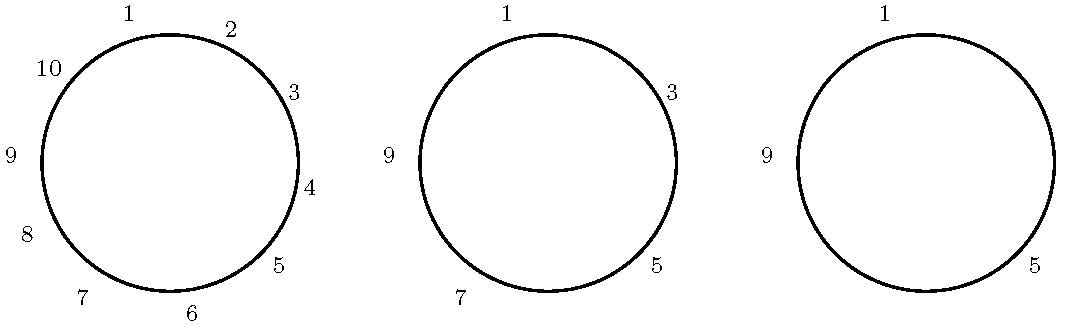
\includegraphics[width=0.5\textwidth]{../../img/josephus-10.jpg}
\caption{\label{fig:orgparagraph1}
n=10的约瑟夫问题}
\end{figure}

消去的顺序是:2,4 6,8,10,3,7,1,9,于是5幸存下来。问题:确定幸存者的号码 \(J(n)\)?

\section{约瑟夫问题递归式}
\label{sec:orgheadline2}


因为有 \(J(10)=5\),所以我们猜测有 \(J(n)= \frac{n}{2}\),但是一些简单的如同下表的例子否定了这个猜测。


\begin{center}
\begin{tabular}{lrrrrrr}
\(n\) & 1 & 2 & 3 & 4 & 5 & 6\\
\hline
\({J_{n}}\) & 1 & 1 & 3 & 1 & 3 & 5\\
\end{tabular}
\end{center}


不过我们可以大胆猜测, \(J(n)\)一定是奇数,因为绕圈走一圈就消去了全部的偶数。如果 \(n\) 是偶数,则走一圈后除了仅剩下一半人口并且他们的号码有变化外,我们面临的情形是与刚开始相同的情形,如下图所示:
\begin{figure}[htb]
\centering
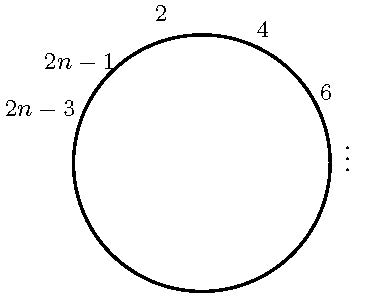
\includegraphics[width=0.3\textwidth]{../../img/josephus-n-even.jpg}
\caption{n为偶数时的约瑟夫问题}
\end{figure}

如此,规模为 \(2n\) 问题就变成了规模为 \(n\) 的问题。这个规模为 \(n\) 的问题与原来相比只是在人员的序号上有所不同,具体说来就是除了每个人的号码加倍并减去1外, \(J(2n)\) 问题和 \(2J(n) -1\)问题没有什么区别。即
\begin{equation}
\label{eq:1}
J(2n) = 2J(n) -1 , n\ge 1
\end{equation}

由上文我们知道 \(J(10)=5\),几乎瞬间我们就会知道 \(J(20)= 2J(10)-1= 2*5 -1 = 9\)。如此可以瞬间解决所有的 \(J(5*2^{m}),m\ge 1\)问题, \(J(5*2^{m}) = 2J(5*2^{m-1}) + 1 = 2*2^{m} +1 = 2^{m+1} +1\),这一步隐含了数学归纳法的证明过程。

假设 \(n\) 是奇数,与偶数不同的情形在于,转第一圈后就把编号为1的人给杀掉了,第二圈开始是从编号为3的人开始的,第二圈开始后第一个要杀掉的人是5。

\begin{figure}[htb]
\centering
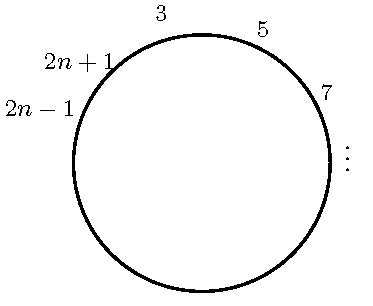
\includegraphics[width=0.3\textwidth]{../../img/josephus-n-odd.jpg}
\caption{n为奇数时的约瑟夫问题}
\end{figure}

如此, \(J(2n+1)\)问题就简化为 \(2J(n)+1\)问题,即:
\begin{equation}
\label{eq:2}
J(2n+1) = 2J(n) +1 , n\ge 1
\end{equation}

综上,约瑟夫问题递归式可以总结为:

\begin{equation}
\label{eq:3}
\begin{split}
J(1)&=1 \\
J(2n)&=2J(n) -1 \\
J(2n+1)&=2J(n)+1
\end{split}
\end{equation}

\section{约瑟夫递归式的解}
\label{sec:orgheadline3}


从约瑟夫递归式可以看出,不同于汉诺塔和披萨饼问题,约瑟夫问题递归式给出的不是 \(J(n)\) 和 \(J(n-1)\) 之间的递归关系,而是 \(J(2n)\) 或者 \(J(2n-1)\) 与 \(J(n)\) 之间的关系。

有了递归式,我们计算一些较小的值


\begin{center}
\begin{tabular}{lrrrrrrrrrrrrrrrr}
\(n\) & 1 & 2 & 3 & 4 & 5 & 6 & 7 & 8 & 9 & 10 & 11 & 12 & 13 & 14 & 15 & 16\\
\hline
\(J_{n}\) & 1 & 1 & 3 & 1 & 3 & 5 & 7 & 1 & 3 & 5 & 7 & 9 & 11 & 13 & 15 & 1\\
\end{tabular}
\end{center}


显然,从上面的表格中可以看出,将 \(n\) 按照 2的幂次进行分组或许会出现一些转机。每一组开始的 \(J(n)\) 总是等于1。仔细观察上表,如果将 \(n\) 写作 \(2^{m}+l\),则 \(J(n)=J(2^{m}+l) = 2l +1, m\ge 0\le l < 2^{m}\). 其中 \(2^{m}\)是不超过 \(n\) 的 \(2\)的最大幂,而 \(l=n-2^{m}\)。事实上,可以对 \(m\) 使用数学归纳法证明:
\begin{equation}
\label{eq:4}
J(n)=J(2^{m}+l) = 2l +1, m\ge 0\le l < 2^{m}
\end{equation}

如此,我们得出了约瑟夫问题的闭式解。对于 \(J(100)\) 因为 \(100=2^{6}+36\),所以 \(J(100)=2*36 +1= 73\)
\section{拓展1:二进制与约瑟夫问题}
\label{sec:orgheadline4}


接下来我们针对约瑟夫问题做一些深入的挖掘。在求解约瑟夫问题递归式闭式解的过程中, \(n\) 和 \(J(n)\) 的以2为基的表示发挥着重要的作用,我们自然要研究以2为基的表示与约瑟夫问题之间的关系。假设 \(n\) 的二进制表示为:
\begin{equation}
\label{eq:5}
n = (b_{m}b_{m-1}\ldots b_{1}b_{0})_{2}
\end{equation}
即, \(n = b_{m}2^{m} + b_{m-1}2^{m-1} + b_{1}2 + b_{0}\),其中 \(b_{i}, i=0,1,\ldots,m-1\) 为 \(0\) 或者 \(1\)。  \(b_{m}=1\),注意 \(n=2^{m}+l\),所以:
\begin{eqnarray}
\label{eq:6}
n & = & (1b_{m-1}\ldots b_{1}b_{0})_{2} \\
l & = & (0b_{m-1}\ldots b_{1}b_{0})_{2} \\
2l& = & (b_{m-1}\ldots b_{1}b_{0}0)_{2} \\
2l+1& = & (b_{m-1}\ldots b_{1}b_{0}1)_{2} \\
J(n) & = & (b_{m-1}\ldots b_{1}b_{0}b_{m})_{2} 
\end{eqnarray}

即,我们得到了:
\begin{equation}
\label{eq:7}
J((b_{m}b_{m-1}\ldots b_{1}b_{0})_{2}) = (b_{m-1}b_{m-2}\ldots b_{1}b_{0}b_{m})_{2}
\end{equation}

在计算机程序设计过程中,只需要对 \(n\) 的二进制表示循环左移1位即可得到 \(J(n)\)!!!这是多么的令人激动啊!在刚开始的时候,我们看约瑟夫问题显得好困难,但是,此刻我们只需要对\(n\) 的二进制表示循环左移1位即可得到 \(J(n)\)!!! 对一个问题深入分析竟然可以得到如此精妙而简洁的答案!高老头不愧是高老头!

还以 \(J(100)\) 为例, 因为 \(100=(1100100)_{2}\),所以 \(J((1100100)_{2}) = (1001001)_{2} = 73\) !!!
\section{拓展2:更一般的约瑟夫递归式}
\label{sec:orgheadline5}


接下来跟进一步深入挖掘该问题,对约瑟夫递归式做更进一步的推广。如下:

\begin{equation}
\label{eq:8}
\begin{split}
 f(1) &= \alpha \\
 f(2n) &= 2f(n) + \beta \\
 f(2n+1) &= 2f(n) + \gamma
\end{split}
\end{equation}

可以看出在约瑟夫问题中, \(\alpha=1,\beta=-1,\gamma=1\)。接下来,我们依然从小入手,得出下表

\begin{center}
\begin{tabular}{rl}
\hline
n & \(f(n)\)\\
1 & \(\alpha\)\\
\hline
2 & 2\(\alpha\)+\(\beta\)\\
3 & 2\(\alpha\)+  +\(\gamma\)\\
\hline
4 & 4\(\alpha\)+3\(\beta\)\\
5 & 4\(\alpha\)+2\(\beta\)+\(\gamma\)\\
6 & 4\(\alpha\)+\(\beta\)+2\(\gamma\)\\
7 & 4\(\alpha\)+  +3\(\gamma\)\\
\hline
8 & 8\(\alpha\)+7\(\beta\)\\
9 & 8\(\alpha\)+6\(\beta\)+\(\gamma\)\\
\hline
\end{tabular}
\end{center}

从上表我们可以看出, \(\alpha\) 的系数是2的幂,且不超过n。 \(\beta\) 的系数则从2的幂减一递减到0,\(\gamma\) 的系数则从0开始递增直到2的幂减一。于是式(\ref{eq:1})的解可以表示为:
\begin{equation}
\label{eq:9}
f(n) = A(n) \alpha + B(n) \beta + C(n) \gamma
\end{equation}

则, \(A(n),B(n),C(n)\)可以分别表示为:
\begin{equation}
\label{eq:10}
\begin{split}
A(n) &= 2^{m} \\
B(n) & = 2^{m} -1 -l \\
C(n) & = l
\end{split}
\end{equation}

其中, \(n = 2^{m}+l, 0\le l < 2^{m},n\ge 1\). 对式(\ref{eq:9})用数学归纳法可以证明。

联想到之前采用二进制表示约瑟夫问题的解:
\begin{equation}
\label{eq:11}
J((b_{m}b_{m-1}\ldots b_{1}b_{0})_{2}) = (b_{m-1}b_{m-2}\ldots b_{1}b_{0}b_{m})_{2}
\end{equation}

\(n\) 的循环左移即是 \(J(n)\) 的解。那么对于式(\ref{eq:11}) 这个更一般的推广,有没有二进制表示呢? 当然有! 首先式(\ref{eq:11}) 可以改写为:
\begin{equation}
\label{eq:12}
\begin{split}
f(1) &=  \alpha \\
f(2n +j) &= 2f(n) +\beta_{j},  j=0,1
\end{split}
\end{equation}
则式(\ref{eq:12})可以改写为:

\begin{equation}
\label{eq:13}
\begin{split}
f((b_{m}b_{m-1}\ldots b_{1}b_{0})_{2}) &=  2f((b_{m}b_{m-1}\ldots b_{2}b_{1})_{2}) + \beta_{b_{0}} \\
&= 4f((b_{m}b_{m-1}\ldots b_{3}b_{2})_{2})+ 2\beta_{b_{1}} + \beta_{b_{0}} \\
&= 8f((b_{m}b_{m-1}\ldots b_{4}b_{3})_{2})+ 4\beta_{b_{2}} + 2\beta_{b_{1}} + \beta_{b_{0}} \\
& \vdots \\
&= 2^{m}f((b_{m})_{2}) + 2^{m-1}\beta_{b_{m-1}} + \ldots + 2\beta_{b_{1}} + \beta_{b_{0}} \\
&= 2^{m} \alpha + 2^{m-1}\beta_{b_{m-1}} + \ldots + 2\beta_{b_{1}} + \beta_{b_{0}} 
\end{split}
\end{equation}

最后,可得:
\begin{equation}
\label{eq:14}
f((b_{m}b_{m-1}\ldots b_{1}b_{0})_{2}) = (\alpha\beta_{b_{m-1}}\beta_{b_{m-2}}\ldots \beta_{b_{1}}\beta_{b_{0}})_{2}
\end{equation}

事实上我们对 \(f(n)\)的前几个解稍加整理即可看出式 (\ref{eq:14}) 的精妙。如下表
\begin{center}
\begin{tabular}{rl}
\hline
n & \(f(n)\)\\
\hline
1 & \(\alpha\)\\
\hline
2 & 2\(\alpha\) +\(\beta\)\\
3 & 2\(\alpha\) +\(\gamma\)\\
\hline
4 & 4\(\alpha\) + 2\(\beta\) + \(\beta\)\\
5 & 4\(\alpha\) + 2\(\beta\) + \(\gamma\)\\
6 & 4\(\alpha\) + 2\(\gamma\)+\(\beta\)\\
7 & 4\(\alpha\) + 2\(\gamma\)+\(\gamma\)\\
\hline
\end{tabular}
\end{center}

在此, 我们有 \(\beta_{0} = \beta , \beta_{1} = \gamma\). 仍然以 \(J(100)\) 为例,因为 \(100 = (1100100)_{2}\), 其解为:

\begin{equation}
\label{eq:15}
(\alpha\beta_{b_{m-1}}\beta_{b_{m-2}}\ldots \beta_{b_{1}}\beta_{b_{0}})_{2} = ( 1 \beta_{1} \beta_{0}\beta_{0} \beta_{1}\beta_{0}\beta_{0})_{2} 
\end{equation} 

因为 \(\alpha = 1, \beta_{0}=\beta = -1, \beta_{1}=\gamma=1\) ,所以 式(\ref{eq:15})可以重写为:
\begin{equation}
\label{eq:16}
( 1 \beta_{1} \beta_{0}\beta_{0} \beta_{1}\beta_{0}\beta_{0})_{2} = (1\quad 1\quad -1\quad -1\quad 1\quad -1\quad -1)_{2} = 73
\end{equation}

注意在此,我们突破了二进制只有0和1的限制,不过这一突破使得约瑟夫的解更加的精炼。
\section{推广3:不同基底的约瑟夫递归式}
\label{sec:orgheadline6}


可以沿着推广2的思路走的更远,我们对式(\ref{eq:12}) 做更进一步修改:
\begin{equation}
\label{eq:17}
\begin{split}
f(j) &=  \alpha_{j}, 1\le j < d \\
f(dn+j)&= c f(n) +\beta_{j}, 0\le j < d 
\end{split}
\end{equation}

式(\ref{eq:17})有变动基数的解:
\begin{equation}
\label{eq:18}
f((b_{m}b_{m-1}\ldots b_{1}b_{0})_{d}) = (\alpha_{b_{m}} \beta_{b_{m-1}} \beta_{b_{m-2}} \ldots \beta_{b_{1}} \beta_{b_{0}})_{c}
\end{equation}
\section{推广4:倒数第二个位置}
\label{sec:orgheadline7}


约瑟夫有一个朋友,他站在倒数第二个位置上因而获救。当每隔一个人就有一个人被处死时,倒数第二个幸存者 \(I(n)\) 的号码是多少?

每隔一个人就有一个人被处死的约瑟夫问题解为:

\begin{equation}
\label{eq:19}
J(n) = J(2^{m} +l) =  2l +1
\end{equation}

此时有: \(2l +1 = n-1 \rightarrow  n=2l +2\) ,满足此式的 \(n\) 总是倒数第二个位置上的人获救。
\end{document}
